\documentclass[aspectratio=169]{../latex_main/tntbeamer}  % you can pass all options of the beamer class, e.g., 'handout' or 'aspectratio=43'
\usepackage{dsfont}
\usepackage{bm}
\usepackage[english]{babel}
\usepackage[T1]{fontenc}
%\usepackage[utf8]{inputenc}
\usepackage{graphicx}
\graphicspath{ {./figures/} }
\usepackage{algorithm}
\usepackage[ruled,vlined,algo2e,linesnumbered]{algorithm2e}
\usepackage{hyperref}
\usepackage{booktabs}
\usepackage{mathtools}

\usepackage{amsmath,amssymb}

\DeclareMathOperator*{\argmax}{arg\,max}
\DeclareMathOperator*{\argmin}{arg\,min}

\usepackage{amsbsy}
\newcommand{\vect}[1]{\bm{#1}}
%\newcommand{\vect}[1]{\boldsymbol{#1}}

\usepackage{pgfplots}
\pgfplotsset{compat=1.16}
\usepackage{tikz}
\usetikzlibrary{trees} 
\usetikzlibrary{shapes.geometric}
\usetikzlibrary{positioning,shapes,shadows,arrows,calc,mindmap}
\usetikzlibrary{positioning,fadings,through}
\usetikzlibrary{decorations.pathreplacing}
\usetikzlibrary{intersections}
\pgfdeclarelayer{background}
\pgfdeclarelayer{foreground}
\pgfsetlayers{background,main,foreground}
\tikzstyle{activity}=[rectangle, draw=black, rounded corners, text centered, text width=8em]
\tikzstyle{data}=[rectangle, draw=black, text centered, text width=8em]
\tikzstyle{myarrow}=[->, thick, draw=black]

% Define the layers to draw the diagram
\pgfdeclarelayer{background}
\pgfdeclarelayer{foreground}
\pgfsetlayers{background,main,foreground}

% Requires XeLaTeX or LuaLaTeX
%\usepackage{unicode-math}

\usepackage{fontspec}
%\setsansfont{Arial}
\setsansfont{RotisSansSerifStd}[ 
Path=../latex_main/fonts/,
Extension = .otf,
UprightFont = *-Regular,  % or *-Light
BoldFont = *-ExtraBold,  % or *-Bold
ItalicFont = *-Italic
]
\setmonofont{Cascadia Mono}[
Scale=0.8
]

% scale factor adapted; mathrm font added (Benjamin Spitschan @TNT, 2021-06-01)
%\setmathfont[Scale=1.05]{Libertinus Math}
%\setmathrm[Scale=1.05]{Libertinus Math}

% other available math fonts are (not exhaustive)
% Latin Modern Math
% XITS Math
% Libertinus Math
% Asana Math
% Fira Math
% TeX Gyre Pagella Math
% TeX Gyre Bonum Math
% TeX Gyre Schola Math
% TeX Gyre Termes Math

% Literature References
\newcommand{\lit}[2]{\href{#2}{\footnotesize\color{black!60}[#1]}}

%%% Beamer Customization
%----------------------------------------------------------------------
% (Don't) Show sections in frame header. Options: 'sections', 'sections light', empty
\setbeamertemplate{headline}{empty}

% Add header logo for normal frames
\setheaderimage{
	% 
\includegraphics[height=\logoheight]{figures/TNT_darkv4.pdf}
	
\includegraphics[height=\logoheight]{../latex_main/figures/luh_logo_rgb_0_80_155.pdf}
	% 
\includegraphics[height=\logoheight]{figures/logo_tntluh.pdf}
}

% Header logo for title page
\settitleheaderimage{
	% 
\includegraphics[height=\logoheight]{figures/TNT_darkv4.pdf}
	
\includegraphics[height=\logoheight]{../latex_main/figures/luh_logo_rgb_0_80_155.pdf}
	% 
\includegraphics[height=\logoheight]{figures/logo_tntluh.pdf}
}

% Title page: tntdefault 
\setbeamertemplate{title page}[tntdefault]  % or luhstyle
% Add optional title image here
%\addtitlepageimagedefault{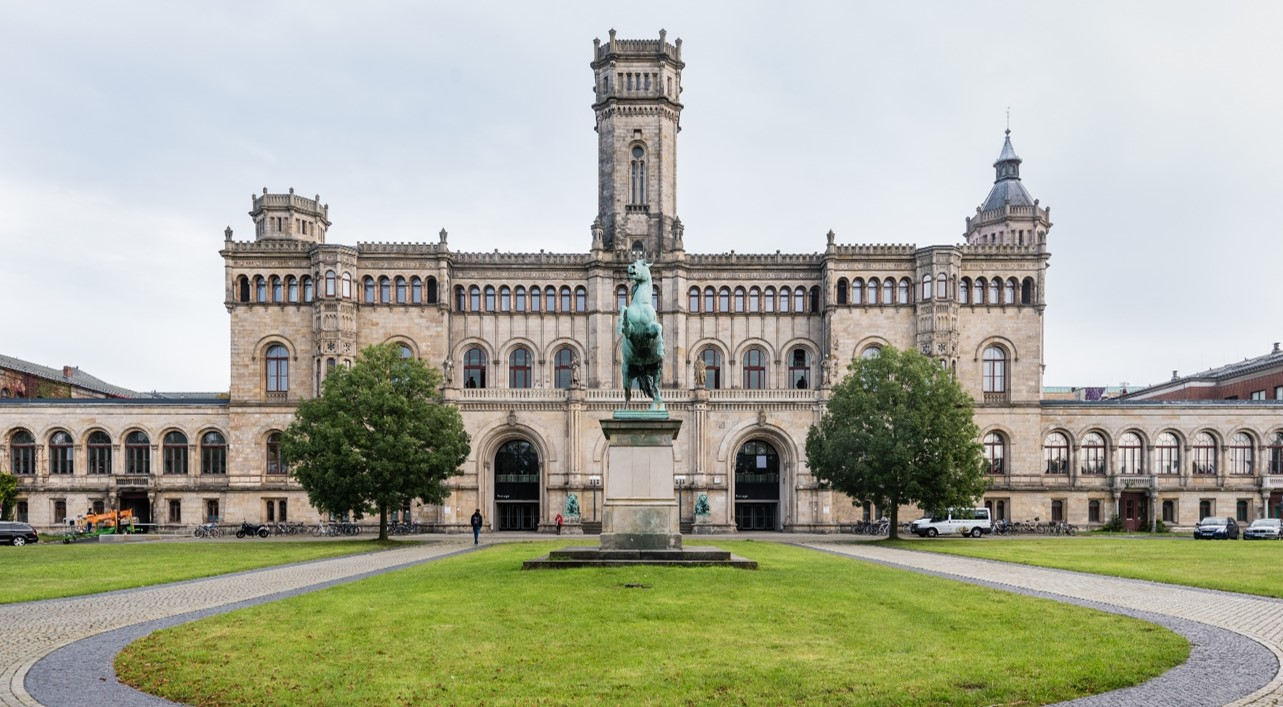
\includegraphics[width=0.65\textwidth]{figures/luh_default_presentation_title_image.jpg}}

% Title page: luhstyle
% \setbeamertemplate{title page}[luhstyle]
% % Add optional title image here
% \addtitlepageimage{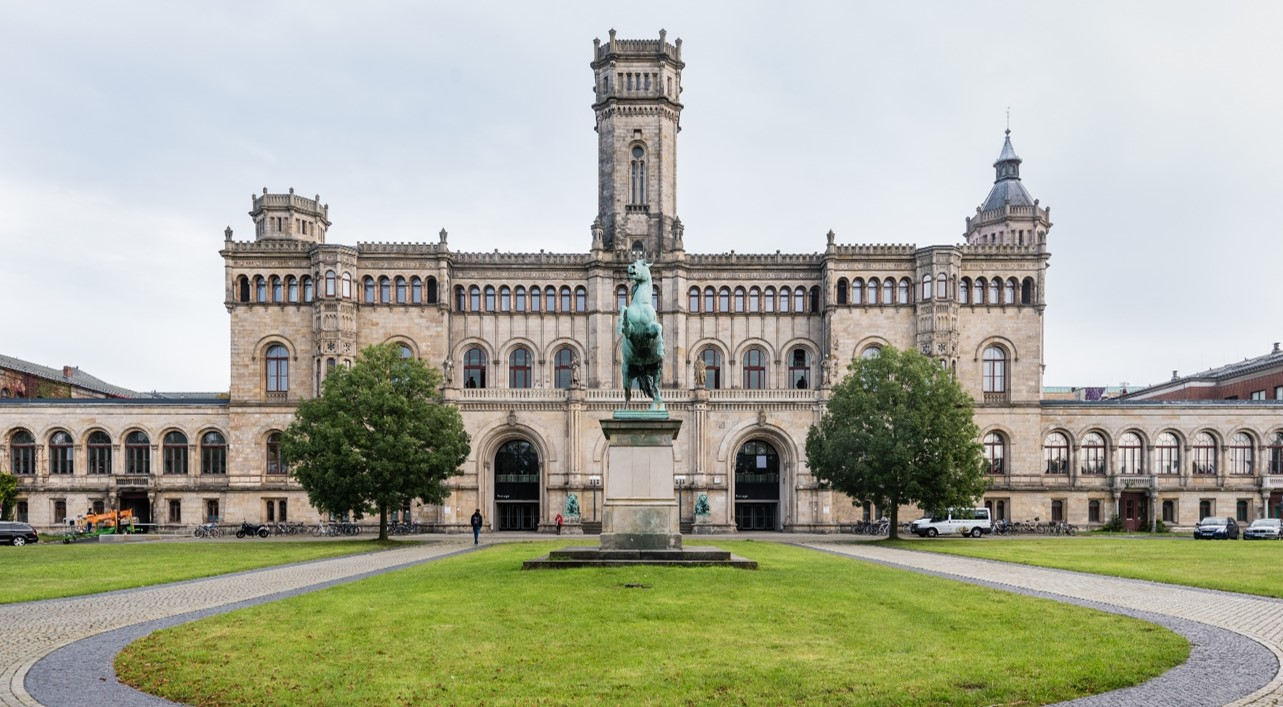
\includegraphics[width=0.75\textwidth]{figures/luh_default_presentation_title_image.jpg}}

\author[Abedjan \& Lindauer]{Ziawasch Abedjan \& Marius Lindauer\\[1em]
	
\includegraphics[height=\logoheight]{../latex_main/figures/luh_logo_rgb_0_80_155.pdf}\qquad
	
\includegraphics[height=\logoheight]{../latex_main/figures/DBIS_Kurzlogo.png}\qquad

\includegraphics[height=\logoheight]{../latex_main/figures/TNT_darkv4}\qquad

\includegraphics[height=\logoheight]{../latex_main/figures/L3S.jpg}	}
\date{Summer Term 2022; \hspace{0.5em} {
\includegraphics[height=1.5em]{../latex_main/figures/Cc-by-nc-sa_icon.svg.png}}; based on \href{https://ds100.org/fa21/}{[DS100]}
}


%%% Custom Packages
%----------------------------------------------------------------------
% Create dummy content
\usepackage{blindtext}

% Adds a frame with the current page layout. Just call \layout inside of a frame.
\usepackage{layout}


%%% Macros
%\renewcommand{\vec}[1]{\mathbf{#1}}
% \usepackage{bm}
%\let\vecb\bm

\title[Classification]{DS: Learning}
\subtitle{Supervised Learning: Classification}

\graphicspath{ {./figure/} }
%\institute{}


\begin{document}
	
    \maketitle
    
    \begin{frame}[c]{What is Classification?}
        \begin{itemize}
            \item Supervised learning considers learning $f: x \mapsto y$ from training data $\mathcal{D}= \{(x_i,y_i)\}_{i}$ 
            \item If $y$ is a category (e.g., ``yes'' vs ''no'') variable we consider it a classification problem
        \end{itemize} 

        \centering
        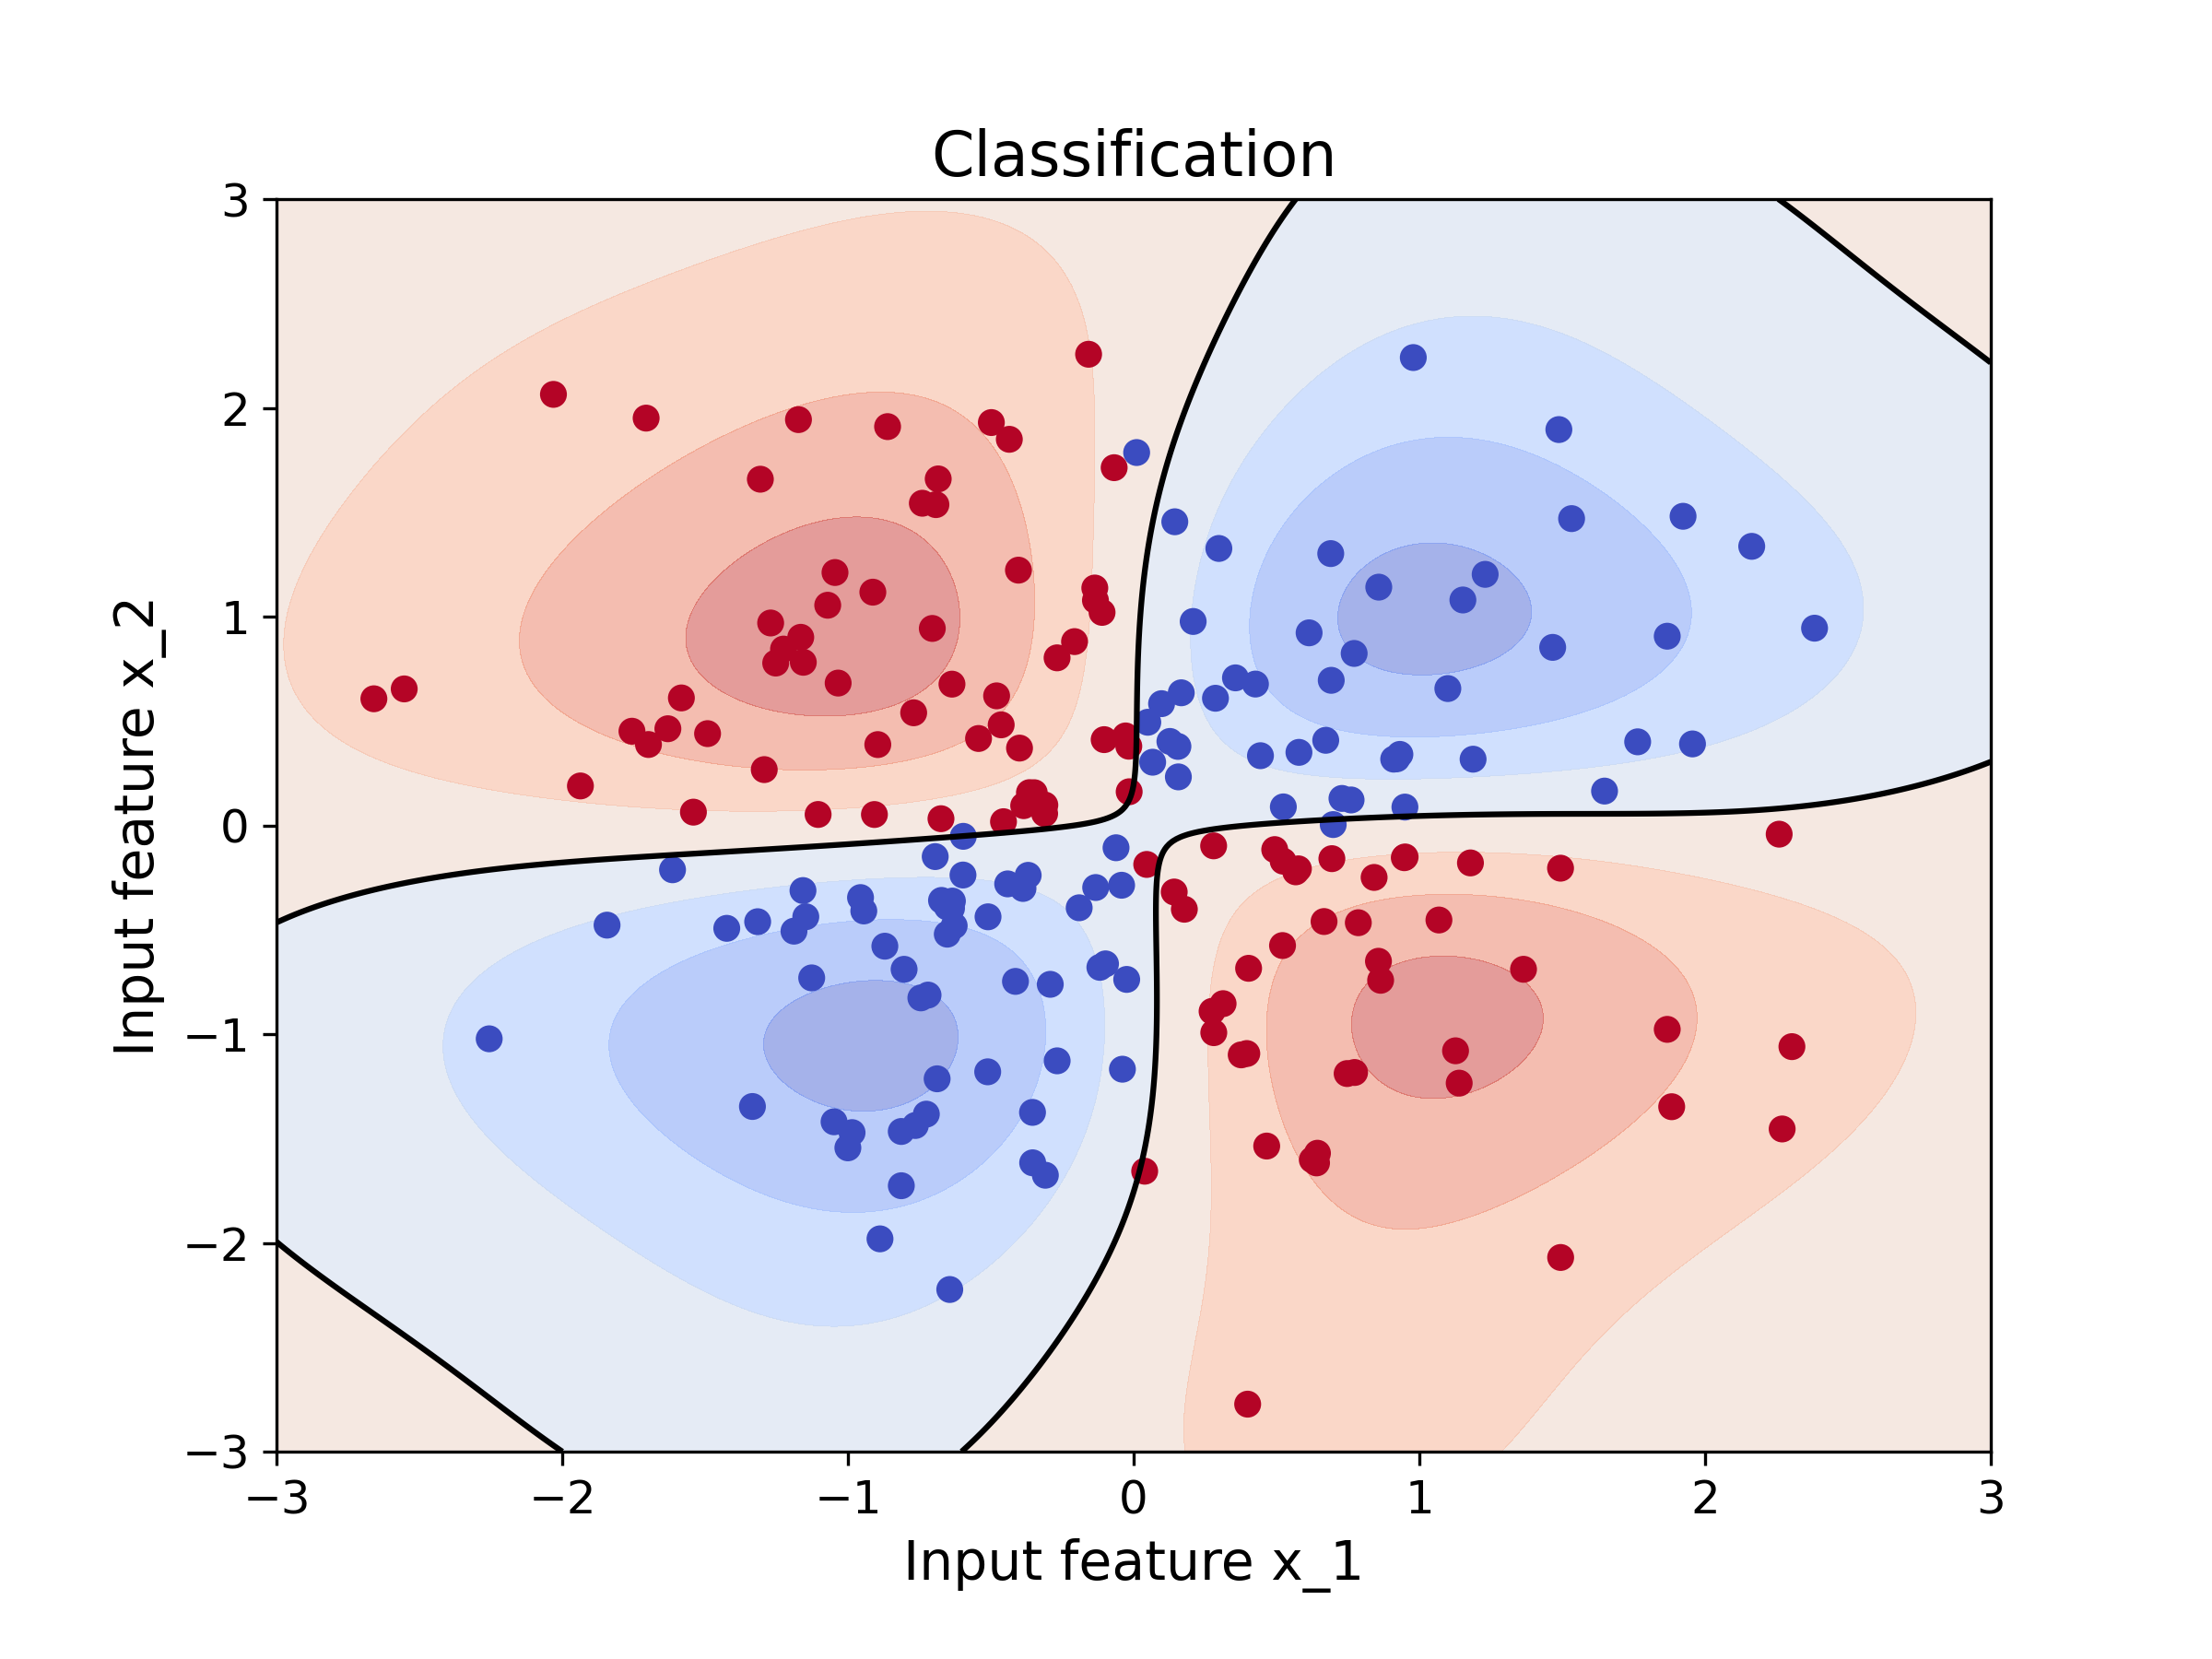
\includegraphics[width=0.5\textwidth]{figure/nonlinear_classification}

    % import numpy as np
    % import matplotlib.pyplot as plt
    % from sklearn import svm
    
    % # Generate random data points
    % np.random.seed(0)
    % X = np.random.randn(200, 2)
    % y = np.logical_xor(X[:, 0] > 0, X[:, 1] > 0)
    
    % # Fit SVM model
    % clf = svm.SVC(kernel='rbf', gamma=0.7, C=1.0)
    % clf.fit(X, y)
    
    % # Create a meshgrid to plot the decision boundary
    % xx, yy = np.meshgrid(np.linspace(-3, 3, 500), np.linspace(-3, 3, 500))
    % Z = clf.decision_function(np.c_[xx.ravel(), yy.ravel()])
    % Z = Z.reshape(xx.shape)
    
    % # Create the plot
    % plt.figure(figsize=(8, 6), dpi=300)
    % plt.contourf(xx, yy, Z, cmap=plt.cm.coolwarm, alpha=0.5)
    % plt.scatter(X[:, 0], X[:, 1], c=y, cmap=plt.cm.coolwarm)
    
    % # Add the classification decision boundary
    % plt.contour(xx, yy, Z, levels=[0], colors='black')
    
    % plt.xlabel('Input feature x_1', fontsize=14)
    % plt.ylabel('Input feature x_2', fontsize=14)
    % plt.xticks(fontsize=12)
    % plt.yticks(fontsize=12)
    % plt.title('Classification', fontsize=16)
    % plt.savefig('nonlinear_classification.png', dpi=300)
    % plt.show()

    \end{frame}

    
    \begin{frame}[c]{Loss Functions}

    \begin{description}
        \item[Cross Entropy] is commonly used in binary classification and multi-class classification problems. For a binary classification problem with a true label $y$ and predicted probability $\hat{p}$, the cross-entropy loss is given by:
        $$\mathcal{L}(y,\hat{p}) = - (y \cdot log(\hat{p}) + (1 - y) \cdot log(1 - \hat{p}))$$

        \item[Hinge Loss] is commonly used in binary classification problems with support vector machines (SVMs). For a binary classification problem with true label $y$ and predicted score $\hat{s}$, the hinge loss is given by
        $$\mathcal{L}(y,\hat{s}) = max(0, 1 - y \cdot \hat{s})$$

        \end{description}
    
    \end{frame}

    \begin{frame}[c]{Classification Models (I)}
        \begin{description}
            \item[Logistic Regression] A statistical model that uses a logistic function to model the probability of a binary outcome given a set of input features.
            \item[Decision Trees] A model that recursively partitions the feature space based on the values of the input features, and assigns a label to each leaf node.
            \item[Random Forests] A randomized ensemble of decision trees
            \item[Support Vector Machines]:  A model that finds a hyperplane that maximally separates the data points of different classes, using a kernel function to map the data into a higher-dimensional space if necessary
        \end{description}

    \end{frame}

    \begin{frame}[c]{Classification Models (II)}
        \begin{description}
            \item[k-Nearest Neighbors (k-NN)] A model that assigns a label to a new data point based on the labels of its k nearest neighbors in the training data.
            \item[Deep Neural Network (DNN)] A model that consists of layers of interconnected neurons, which apply an activation function to a weighted sum of their inputs, and can learn complex non-linear relationships between the input features and the labels.
            \item[Gradient Boosting Machine] A model that uses an ensemble of weak decision trees, and trains them iteratively to improve their accuracy and reduce bias.
            \item[XGBoost] An advanced implementation of gradient boosting that combines tree-based models and regularization techniques to achieve high accuracy and low overfitting.
        \end{description}

    \end{frame}



\end{document}